\let\lesson\undefined
\newcommand{\lesson}{\phantomlesson{Bài 7.}}
\setcounter{section}{2}
\section{Bài tập trắc nghiệm}
\begin{enumerate}[label=\bfseries Câu \arabic*:]
	\item \mkstar{1}\\
	{Gia tốc là một đại lượng
	\begin{mcq}
		\item đại số, đặc trưng cho sự biến thiên nhanh hay chậm của chuyển động.
		\item đại số, đặc trưng cho tính không đổi của vận tốc.
		\item vectơ, đặc trưng cho sự biến thiên nhanh hay chậm của chuyển động.
		\item vectơ, đặc trưng cho sự biến thiên nhanh hay chậm của vận tốc.
	\end{mcq}
}
\hideall{
\textbf{Đáp án: D.}
}

\item \mkstar{1}\\
{Chọn ý sai. Khi một chất điểm chuyển động thẳng biến đổi đều thì nó
\begin{mcq}
	\item có gia tốc không đổi.
	\item có tốc độ tức thời tăng đều hoặc giảm đều theo thời gian.
	\item có gia tốc tăng dần đều theo thời gian.
	\item có thể lúc đầu chậm dần đều, sau đó nhanh dần đều.
\end{mcq}

}
\hideall{
\textbf{Đáp án: B.}
}

\item \mkstar{2}\\
{Chọn phát biểu sai.
	\begin{mcq}
		\item Trong chuyển động thẳng biến đổi đều, quãng đường đi được trong những khoảng thời gian bằng nhau thì bằng nhau.
		\item Gia tốc của chuyển động thẳng biến đổi đều có độ lớn không đổi.
		\item Vectơ gia tốc của chuyển động thẳng biến đổi đều có thể cùng chiều hoặc ngược chiều với vectơ vận tốc.
		\item Vận tốc tức thời của chuyển động thắng biến đổi đều có độ lớn tăng hoặc giảm đều theo thời gian.
	\end{mcq}

}
\hideall{
\textbf{Đáp án: A.}
}

\item \mkstar{2}\\
{Để đặc trưng cho chuyển động về sự nhanh, chậm và về phương chiều, người ta đưa ra khái niệm
\begin{mcq}(2)
	\item vectơ gia tốc tức thời.
	\item vectơ gia tốc trung bình.
	\item vectơ vận tốc tức thời.
	\item vectơ vận tốc trung bình.
\end{mcq}
}
\hideall{
\textbf{Đáp án: C.}
}

\item \mkstar{3}\\
{\begin{minipage}[l]{0.7\textwidth}
		Một chất điểm chuyển động thẳng đều, với đồ thị vận tốc - thời gian được cho như hình vẽ. Quãng đường mà chất điểm đi được trong khoảng thời gian từ 1 s đến 2 s là
		\begin{mcq}(2)
			\item $\SI{1}{\meter}$.
			\item $\SI{2}{\meter}$.
			\item $\SI{3}{\meter}$.
			\item $\SI{4}{\meter}$.
		\end{mcq}
	\end{minipage}
	\begin{minipage}{0.3\textwidth}
		\begin{center}
			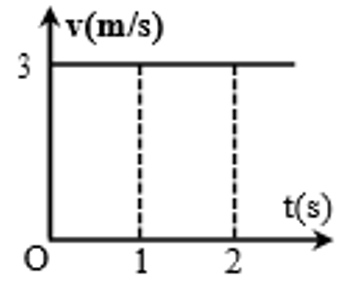
\includegraphics[width=0.7\linewidth]{../figs/VN10-2022-PH-TP008-P-1}
		\end{center}
	\end{minipage}
}
\hideall{
	\textbf{Đáp án: C.}
}

\item \mkstar{3}\\
{\begin{minipage}[l]{0.7\textwidth}
		Đồ thị vận tốc – thời gian của một vật chuyển động thẳng ở hình dưới. Quãng đường vật đã đi được sau $\SI{30}{\second}$ là
		\begin{mcq}(2)
			\item $\SI{200}{\meter}$.
			\item $\SI{250}{\meter}$.
			\item $\SI{300}{\meter}$.
			\item $\SI{350}{\meter}$.
		\end{mcq}
	\end{minipage}
	\begin{minipage}{0.3\textwidth}
		\begin{center}
			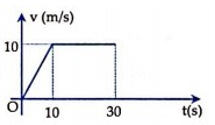
\includegraphics[width=1.0\linewidth]{../figs/VN10-2022-PH-TP008-P-2}
		\end{center}
	\end{minipage}
}
\hideall{
	\textbf{Đáp án: B.}
}

\item \mkstar{3}\\
{\begin{minipage}[l]{0.7\textwidth}
		Đồ thị vận tốc - thời gian của một vật chuyển động được biểu diễn như hình vẽ. Gọi $a_1$, $a_2$, $a_3$ lần lượt là gia tốc của vật trong các giai đoạn tương ứng là từ $t = 0$ đến $t_1 = \SI{20}{\second}$; từ $t_1 =\SI{20}{\second}$ đến $t_2 =\SI{60}{\second}$; từ $t_2 = \SI{60}{\second}$ đến $t_3 = \SI{80}{\second}$. Giá trị của $a_1, a_2, a_3$ lần lượt là
		\begin{mcq}(2)
			\item $\SI{-1}{\meter/\second^2}$; $\SI{0}{\meter/\second^2}$; $\SI{2}{\meter/\second^2}$.
			\item $\SI{1}{\meter/\second^2}$; $\SI{0}{\meter/\second^2}$; $\SI{22}{\meter/\second^2}$.
			\item $\SI{-1}{\meter/\second^2}$; $\SI{2}{\meter/\second^2}$; $\SI{0}{\meter/\second^2}$.
			\item $\SI{1}{\meter/\second^2}$; $\SI{0}{\meter/\second^2}$; $\SI{2}{\meter/\second^2}$.
		\end{mcq}
	\end{minipage}
	\begin{minipage}{0.3\textwidth}
		\begin{center}
			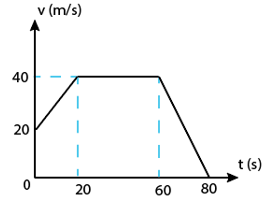
\includegraphics[width=1.0\linewidth]{../figs/VN10-2022-PH-TP008-P-5}
		\end{center}
	\end{minipage}
}
\hideall{
	\textbf{Đáp án: B.}
}

\item \mkstar{3}\\
{\begin{minipage}[l]{0.7\textwidth}
		Đồ thị vận tốc - thời gian của một vật chuyển động được biểu diễn như hình vẽ. Quãng đường vật đi được từ thời điểm $t = 0$ đến thời điểm $t = \SI{60}{\second}$ là
		\begin{mcq}(2)
			\item $\SI{2.2}{\kilo\meter}$.
			\item $\SI{1.1}{\kilo\meter}$.
			\item $\SI{0.44}{\kilo\meter}$.
			\item $\SI{1.2}{\kilo\meter}$.
		\end{mcq}
	\end{minipage}
	\begin{minipage}{0.3\textwidth}
		\begin{center}
			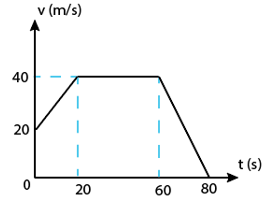
\includegraphics[width=1.0\linewidth]{../figs/VN10-2022-PH-TP008-P-5}
		\end{center}
	\end{minipage}
}
\hideall{
	\textbf{Đáp án: A.}
}
\item \mkstar{4}\\
{\begin{minipage}[l]{0.7\textwidth}
		Hình bên là đồ thị vận tốc - thời gian của hai vật chuyển động thẳng cùng hướng, xuất phát từ cùng một vị trí, gốc thời gian là lúc hai vật bắt đầu chuyển động. Nhận xét sai là
		\begin{mcq}
			\item Hai vật cùng chuyển động nhanh dần.
			\item Vật 1 bắt đầu chuyển động từ trạng thái nghỉ.
			\item Vật 2 chuyển động với gia tốc lớn hơn vật 1.
			\item Ở thời điểm $t_0$, vật 1 ở phía sau vật 2.
		\end{mcq}
	\end{minipage}
	\begin{minipage}{0.3\textwidth}
		\begin{center}
			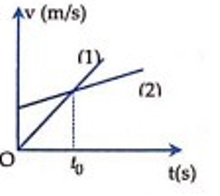
\includegraphics[width=0.8\linewidth]{../figs/VN10-2022-PH-TP008-P-4}
		\end{center}
	\end{minipage}
}
\hideall{
	\textbf{Đáp án: C.}
}

\item \mkstar{4}\\
{\begin{minipage}[l]{0.7\textwidth}
		Đồ thị vận tốc - thời gian của một vật chuyển động như hình bên. Tỉ số về độ lớn gia tốc của vật trong thời gian $OA$ và $AB$ là
		\begin{mcq}(2)
			\item $\dfrac{1}{2}$.
			\item $1$.
			\item $\dfrac{1}{3}$.
			\item $3$.
		\end{mcq}
	\end{minipage}
\begin{minipage}{0.3\textwidth}
	\begin{center}
		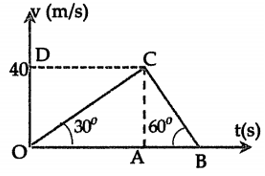
\includegraphics[width=0.8\linewidth]{../figs/VN10-2022-PH-TP008-P-7}
	\end{center}
\end{minipage}
}
\hideall{
\textbf{Đáp án: C.}
}
\end{enumerate}
\section{Bài tập tự luận}
\begin{enumerate}[label=\bfseries Bài \arabic*:]
	\item \mkstar{2}\\
	{Một tài xế xe tải đang chuyển động đều với tốc độ cho phép trên đường cao tốc trong khoảng thời gian $\Delta t$. Khi nhìn thấy biển báo "Đoạn đường hay xảy ra tai nạn", tài xế quyết định giảm tốc độ. Sau khoảng thời gian $\Delta t_1$, tài xế quan sát thấy một tai nạn đột ngột xảy ra ở phía trước. Do đó tài xế hãm phanh gấp để dừng lại trong khoảng thời gian ngắn $\Delta t_2$ để tránh va chạm. Giả sử trong suốt quá trình chuyển động, xe tải luôn chạy trên đường thẳng.
		\begin{enumerate}[label=\alph*)]
			\item Vẽ đồ thị vận tốc - thời gian biểu diễn quá trình chuyển động của xe tải.
			\item Độ dốc của đồ thị trong trường hợp nào lớn nhất?
		\end{enumerate}
}
\hideall{
\begin{enumerate}[label=\alph*)]
	\item \begin{center}
		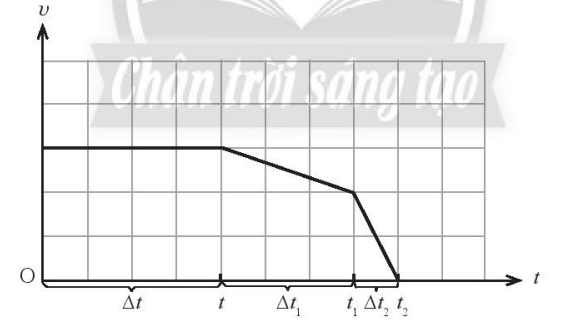
\includegraphics[width=0.4\linewidth]{../figs/VN10-2022-PH-TP008-P-9}
	\end{center}
\item Trong thời gian $\Delta t_2$ độ dốc của đồ thị vận tốc - thời gian là lớn nhất.
\end{enumerate}
}
	
	\item \mkstar{3}
	
	
	{Một vật chuyển động có đồ thị $(v-t)$ như hình bên.
		\begin{center}
			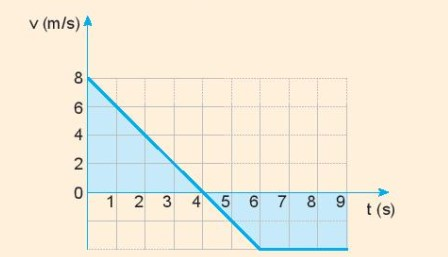
\includegraphics[scale=1]{../figs/VN10-2022-PH-TP012-4.jpg}
		\end{center}
		\begin{enumerate}[label=\alph*)]
			\item Mô tả chuyển động của vật.
			\item Tính độ dịch chuyển trong 4 giây đầu, 2 giây tiếp theo và 3 giây cuối.
			\item Tính gia tốc của chuyển động trong 4 giây đầu.
			\item Tính gia tốc của chuyển động từ giây thứ 4 đến giây thứ 6.
		\end{enumerate}
		
	}
	
	\hideall
	{	\begin{enumerate}[label=\alph*)]
			\item 
			\begin{itemize}
				\item Trong 4 giây đầu tiên: chuyển động chậm dần đều từ  $\SI{8}{m/s}$ đến  $\SI{0}{m/s}$.
				\item Từ giây thứ 4 đến giây thứ 6: bắt đầu tăng tốc với vận tốc  $- \SI{2}{m/s}$.
				\item Từ giây thứ 6 đến giây thứ 9: chuyển động thẳng đều với vận tốc $- \SI{2}{m/s}$.
			\end{itemize}
	\item 
	\begin{itemize}
		\item Trong 4 giây đầu:
		
		Độ dịch chuyển bằng diện tích tam giác vuông có cạnh đáy là $t$ và chiều cao là $v$.
		
		$$d_1 = \dfrac{1}{2}v_1t_1 = \SI{16}{m}.$$
		\item Trong 2 giây tiếp theo:
		
		Độ dịch chuyển bằng diện tích tam giác vuông có cạnh đáy là $t$ và chiều cao là $v$.
		
		$$d_2 = \dfrac{1}{2}v_2t_2 = -\SI{4}{m}.$$
		\item Trong 3 giây cuối:
		
		Độ dịch cuyển bằng diện tích hình chữ nhật có chiều dài là $t$ và chiều rộng là $v$.
		
		$$d_3 = \dfrac{1}{2}v_3t_3 = -\SI{12}{m}.$$
	\end{itemize}
\item Gia tốc của chuyển động trong 4 giây đầu

$$a = \dfrac{\Delta v}{\Delta t} =\dfrac{8 - 0}{4-0}= \SI{2}{m/s}^2.$$
\item Gia tốc của chuyển động từ giây thứ 4 đến giây thứ 6:

$$a = \dfrac{\Delta v}{\Delta t} =\dfrac{-4 - 0}{6-4}= -\SI{2}{m/s}^2.$$
		\end{enumerate}
		
	}
	
	\item \mkstar{3}\\
	{Chuyển động của một vật có đồ thị vận tốc theo thời gian như hình vẽ. Tổng quãng đường vật đã đi bằng bao nhiêu?
		\begin{center}
			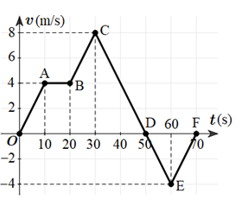
\includegraphics[width=0.3\linewidth]{../figs/VN10-2022-PH-TP008-P-8}
		\end{center}
	
}
\hideall{
$s=\SI{240}{\meter}$.
}

\item \mkstar{3}\\
{Một quả bóng bàn được bắn ra theo phương ngang với vận tốc ban đầu bằng không đến va chạm vào tường và bật lại trong khoảng thời gian rất ngắn. Hình bên là đồ thị $\left(v-t\right)$ mô tả chuyển động của quả bóng trong $\SI{20}{\second}$ đầu tiên. Tính quãng đường mà quả bóng bay được sau $\SI{20}{\second}$ kể từ lúc bắt đầu chuyển động.
	\begin{center}
		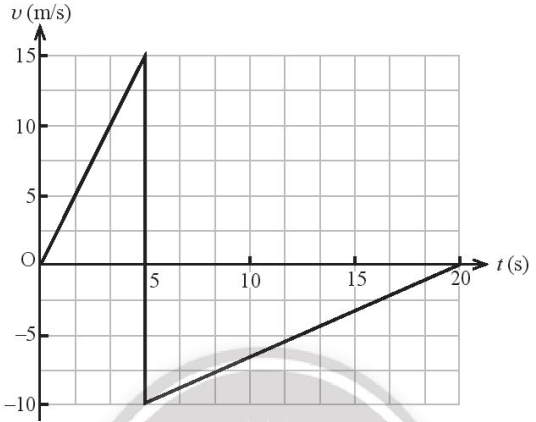
\includegraphics[width=0.4\linewidth]{../figs/VN10-2022-PH-TP008-P-10}
	\end{center}

}
\hideall{
$s=\SI{112.5}{\meter}$.
}
\end{enumerate}